\subsection{Reguladores \quotemarks{low drop-out} (\textbf{LDO})}

La tensión dropout es la mínima diferencia de tensión entre la entrada y la salida dentro de la cual el circuito es todavía capas de regular la salida dentro de las especificaciones. En el regulador estudiado vemos que es aproximadamente $2.23 \si[per-mode=symbol]{\volt}$ ($V_{i} = 12.23 \si[per-mode=symbol]{\volt}$, $V_{o} = 10 \si[per-mode=symbol]{\volt}$, para $R_{L} = 10 \si[per-mode=symbol]{\ohm}$).\\
Un $18.2 \%$ de caída de tensión para regular, puede ser excesivo en determinadas aplicaciones. Por ejemplo, cuando una batería de iones de litio cae de $4.2 V$ (totalmente cargada) a $2.7 \si[per-mode=symbol]{\volt}$ (casi descargada), un \textbf{LDO} puede mantener constantes $2.5 \si[per-mode=symbol]{\volt}$ en la carga.
En un regulador \textbf{LDO} la caída de tensión típica es de $300 \si[per-mode=symbol]{\milli\volt}$.


\subsubsection{Topologías disponibles}

Los \textbf{LDO} se pueden clasificar según el tipo de dispositivo de paso que se use. Sus diferentes estructuras y características ofrecen varias ventajas e inconvenientes.
En la siguiente figura  se muestran ejemplos de cuatro tipos de dispositivos de paso, incluidos los transistores bipolares \textbf{NPN} y \textbf{PNP}, los circuitos Darlington y los transistores \textbf{PMOS}.


\begin{figure}[H] %htb
\begin{center}
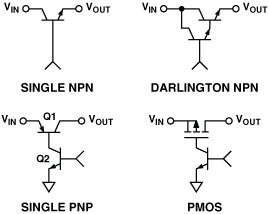
\includegraphics[width=0.6 \textwidth, angle=0]{./img/reguladores/topologies.png}
\caption{\label{fig:fig_sziklai_cir_1}\footnotesize{Topologías de reguladores \textbf{LDO}}}
\end{center}
\end{figure}


Para una tensión de alimentación dada, los dispositivos de paso bipolar pueden entregar la corriente de salida más alta. Se prefiere un \textbf{PNP} a un \textbf{NPN}, porque la base de la \textbf{PNP} se puede conectar a tierra, saturando completamente el transistor si es necesario. La base del \textbf{NPN} solo se puede conectar tan alto como la tensión de alimentación, limitando la caída de tensión mínima a un $V_{be}$. Por lo tanto, los dispositivos de paso \textbf{NPN} y Darlington no pueden proporcionar caídas de voltaje por debajo de $1 \si[per-mode=symbol]{\volt}$. Sin embargo, pueden ser valiosos, cuando se necesita un gran ancho de banda, e inmunidad a la carga capacitiva (gracias a su $Z_{o}$ baja).\\
Los transistores \textbf{PMOS} y \textbf{PNP} pueden saturarse de manera efectiva, minimizando la pérdida de voltaje y la potencia disipada por el dispositivo de paso, lo que permite una baja caída de tensión y una alta eficiencia. Los dispositivos de paso \textbf{PMOS} pueden proporcionar la menor caída de voltaje posible, aproximadamente $r_{DS_{ON}} \cdot I_{L}$, siendo $I_{L}$ la corriente por la carga. También permiten minimizar el flujo de la corriente de reposo. El principal inconveniente es que el transistor \textbf{MOS} es a menudo un componente externo, especialmente para controlar altas corrientes, por lo que convierte al circuito integrado en un controlador, en lugar de ser un regulador autónomo completo. \\
La potencia disipada en el regulador es:

\begin{equation*}
PD = \left( V_{in} - V_{out} \right) \cdot I_{L} + V_{in} \cdot I_{g}
\end{equation*}


El primer término es la disipación del dispositivo de paso, el segundo término es el consumo de energía de la parte del controlador del circuito. La corriente a común, $I_{g}$, en algunos reguladores, especialmente aquellos que usan transistores bipolares saturables como dispositivos de paso, puede alcanzar su pico durante el encendido.\\
En el \textbf{LDO} \textit{LM2931} para $5 \si[per-mode=symbol]{\volt}$, encontramos una impedancia de salida de $200 \si[per-mode=symbol]{\milli\ohm}$, mucho mayor que los $17 \si[per-mode=symbol]{\milli\ohm}$ del \textit{LM7805} (no \textbf{LDO}).












\clearpage